\normalfont\documentclass[letterpaper,11pt]{article}
\usepackage{amsmath, amsfonts,amssymb,latexsym}
\usepackage{fullpage}
\usepackage{parskip}
\usepackage{flexisym}
\usepackage{indentfirst}
\usepackage{graphicx}
\usepackage{algorithm2e}
% \usepackage{algorithm}
\usepackage{algorithmicx}
% \usepackage{algpseudocode}
\usepackage{amsmath}
\begin{document}
\setlength{\parindent}{2ex}
\newcommand{\header}{
	\noindent \fbox{
	\begin{minipage}{6.4in}
	\medskip
	\textbf{CS 271 -  Introduction to Artificial Intelligence} \hfill \textbf{Fall 2016} \\[1mm]
	\begin{center}
		{\Large HomeWork 2} \\[3mm]
	\end{center}
	  Name: \itshape{Liangjian Chen} \\
	  \textnormal{ID}: \itshape{\#52006933} \hfill \today
	\medskip
	\end{minipage}}
}
\bigskip
\header

\begin{enumerate}
\item[Problem 1]\textbf{Solution:}\par
	\begin{enumerate}
		\item
		\item Maximum depth is 9(if the depth of root is $0$).
		\item The graph is below\par
	\end{enumerate}
	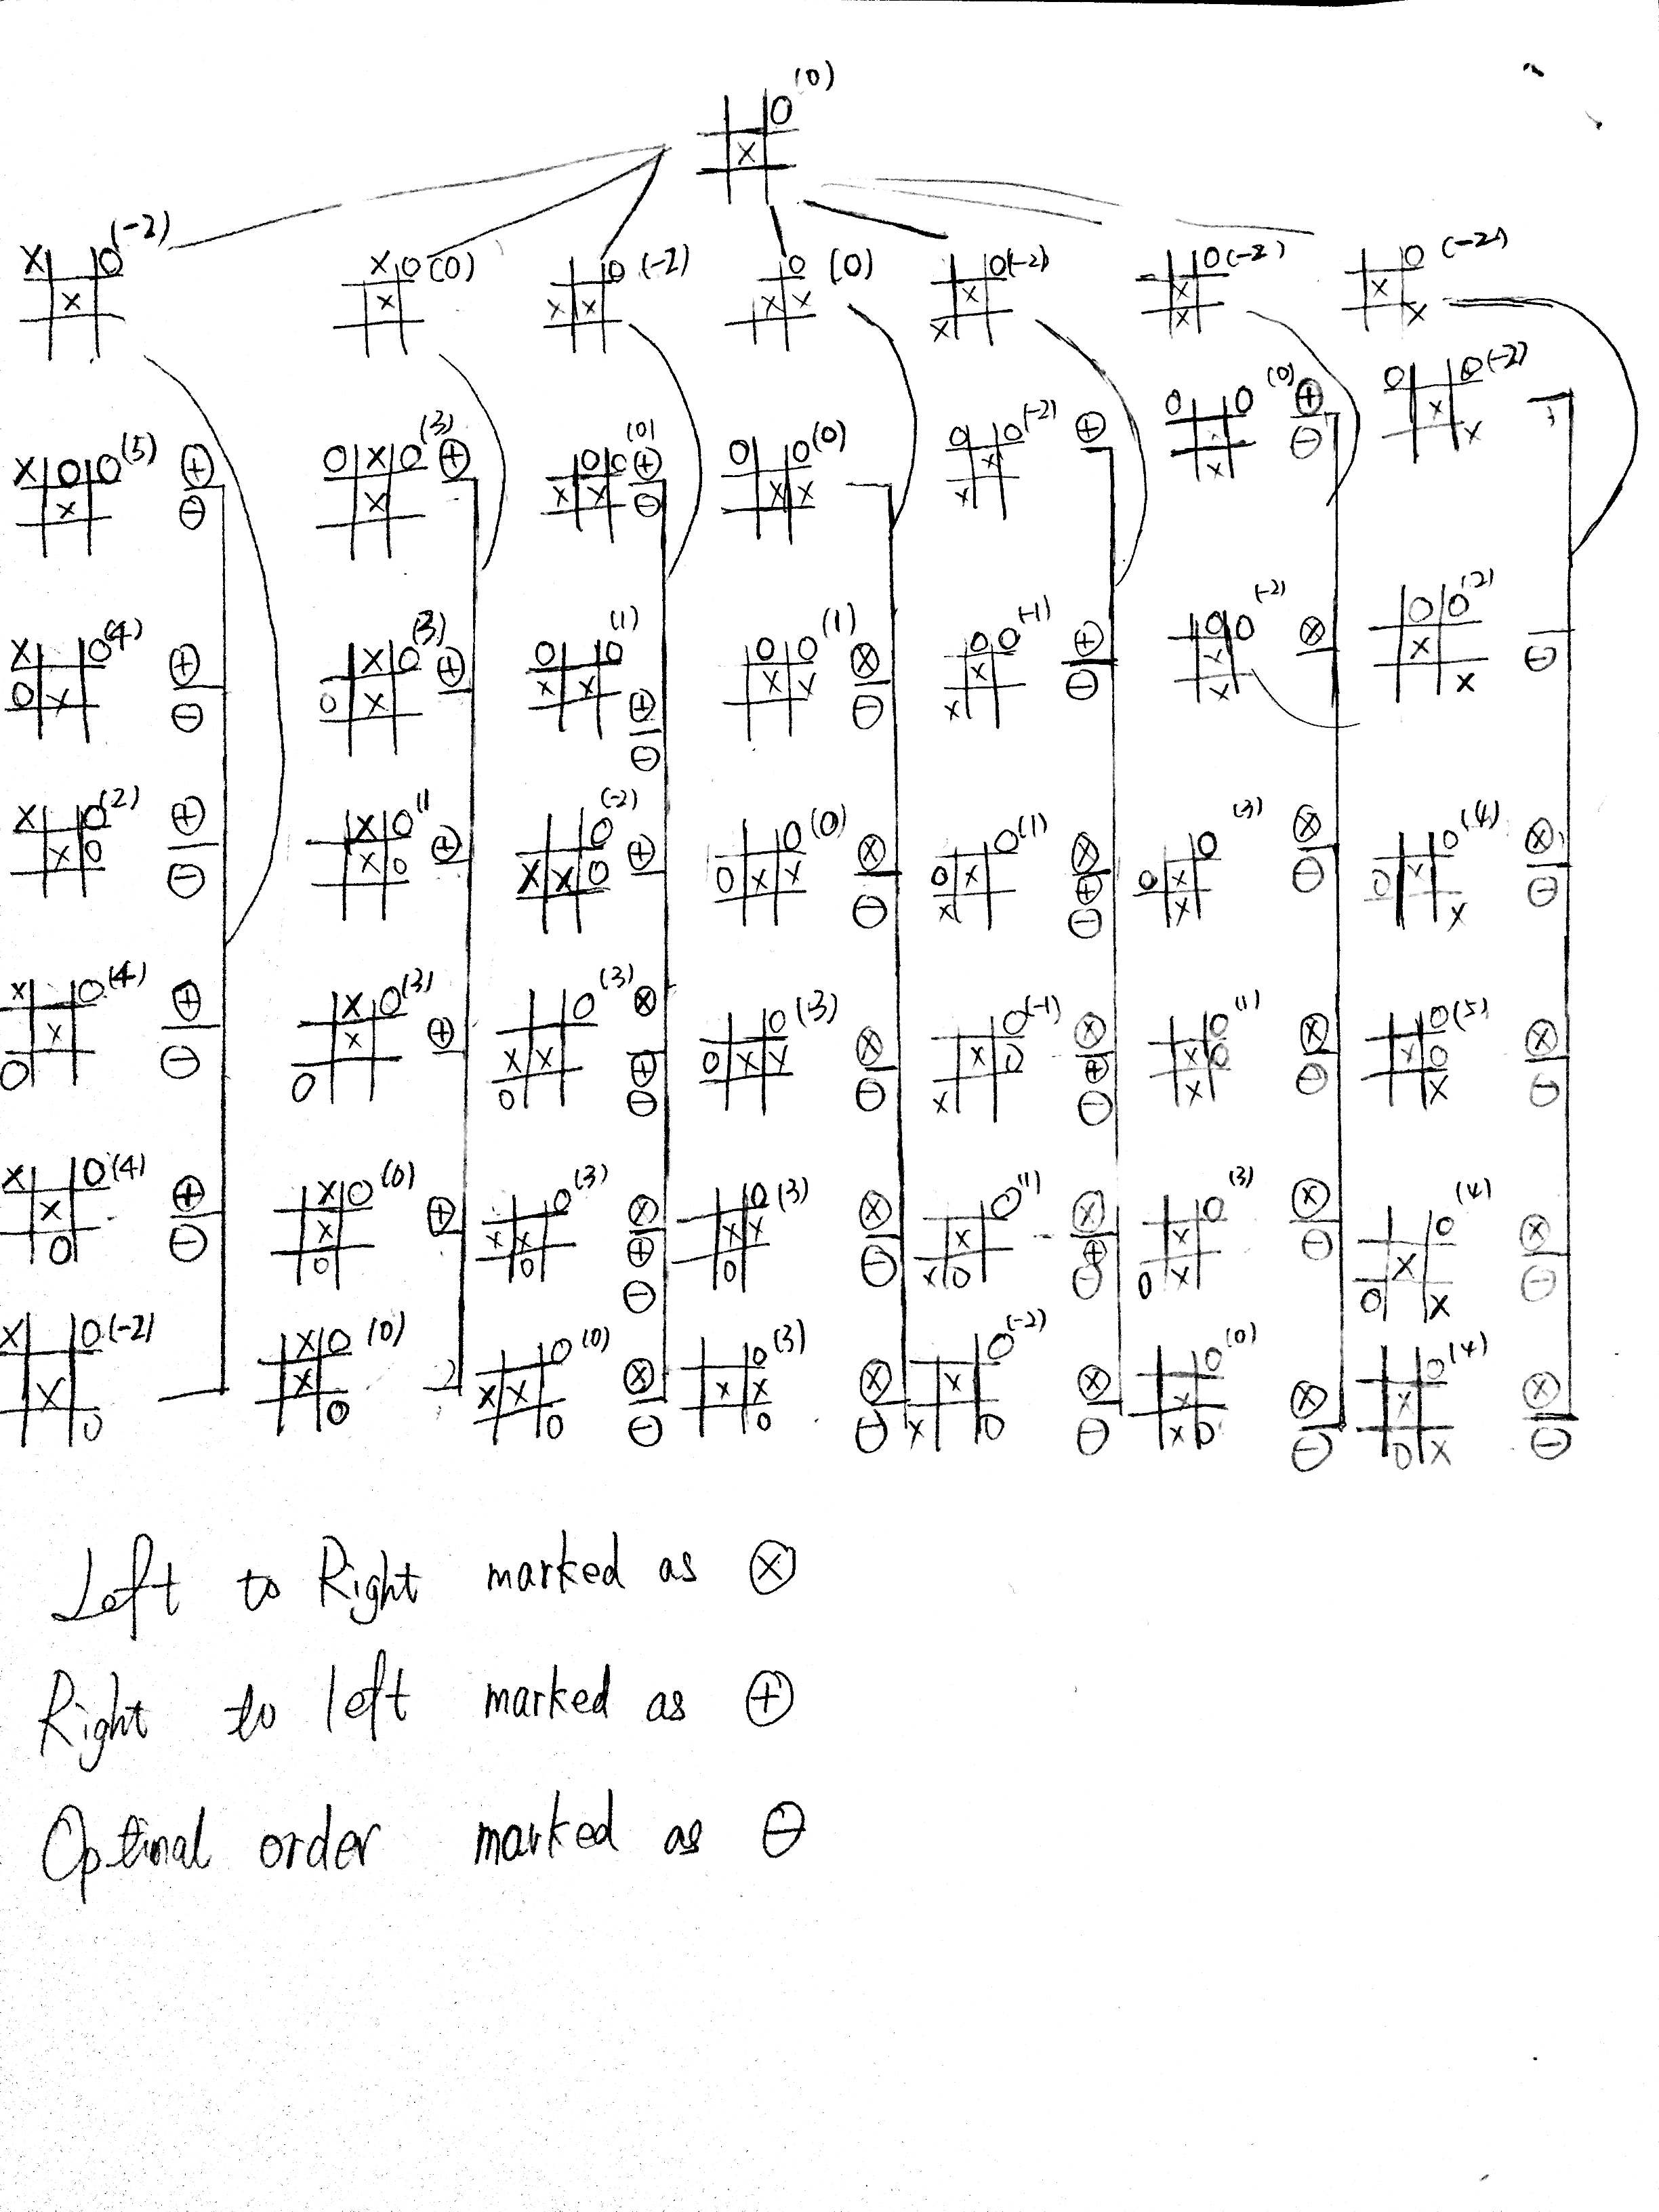
\includegraphics[width=0.72\linewidth]{1.jpg}
	
\item[Problem 2]\textbf{Solution:}\par
	Yes, consider the following evaluation function $f$, $f(x) = 1$, if $x$ is a winning state, $f(x) = -1$ if $x$ is a lost state, and $f(x) = 0$ if $x$ is a tie state. Applied $f(x)$ into this game, then we can use min-max algorithm in this game tree . Thus alpha-beta pruning can correctly applied in this problem.
\item [Problem 3]\textbf{Solution:}\par
	\begin{enumerate}
		\item move to $B$
		\item $O$, $Q$,$I$,$T$.$U$
	\end{enumerate}	
\item[Problem 4]\textbf{Solution:}\par
	Assume $f(x) = 2ax + b$ where $a > 0$.\\
	Because $f(x)$ monotonic incresing, $\forevery x_1,x_2, x_1 > x_2$, $f(x_1)> f(x_2)$. So, the larger value remains after trasforming. Thus choice remains unchanged.
\item [Problem 5]\textbf{Solution:}\par


\end{enumerate}
\end{document}
